%\vspace{-4mm}

\section{Empirical Results on Pre-trained DNNs}
\label{sxn:emp}

\michael{Charles, would you do a core-dump of text for this section, describing the details of the setup and results, and also fill in tables, and I can make a smoothing pass.}

%%\nred{TOO LONG for a 10 page paper...move extra results to  Appendix}

(((
\charles{
In this study, we only need to consider Linear and 2D Convolutional (Conv2D) layers because we will only examine series of commonly
available, open source, pre-trained DNNs with these kinds of layers.  We describe these pre-trained models in detail below;
briefly examine the VGG series (VGG11, VGG13, VGG1, VGG19), with and without BatchNorm, the complete set of
available ResNet models ranging from ResNet10 to ResNet152(b), and a wide range of other models.  All models have
been trained on ImageNet, and reported test accuracies are available.  For our analysis, we do not needs to retrain these
models, and we do not even need access to the test data.  }
)))

(((
As illustrated in Figure~\ref{fig:vgg_lognorms}, this 
(average log norm of the weight matrices of Eqn.~(\ref{eqn:av_log_norm}))
metric is a relatively good complexity metric for comparing the test accuracies of different, pre-trained DNNs in the same series.
)))


\paragraph{VGG and VGG\_BN Models.}

\begin{figure}[t] %[!htb]
   \centering
   \subfigure[log Frobenius norm $\langle\log\Vert\mathbf{W}\Vert_{F}\rangle$]{
      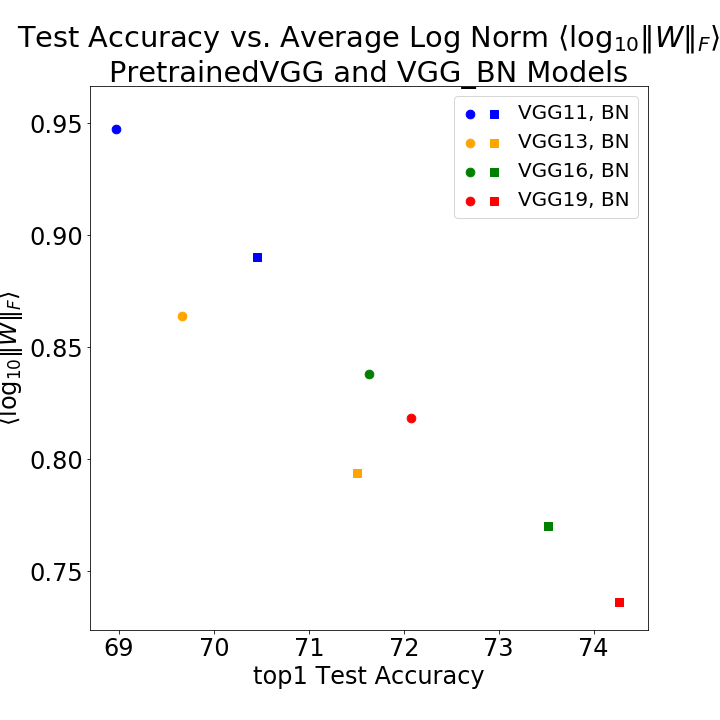
\includegraphics[scale=0.35]{img/vgg-lognorms.png}
      \label{fig:vgg_lognorms}
   }
   \subfigure[weighted average PL exponent $\hat{\alpha}$]{
      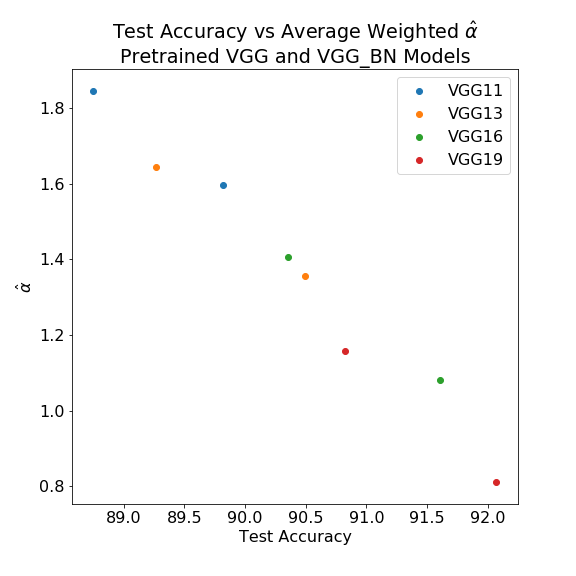
\includegraphics[scale=0.35]{img/vgg-w_alphas.png}
      \label{fig:vgg_alphahat}
   }
   \caption{%
      Pre-trained VGG and VGG\_BN Architectures and DNNs.  
      Test Accuracy versus
      average log Frobenius norm $\langle\log\Vert\mathbf{W}\Vert_{F}\rangle$ (in (\ref{fig:vgg_lognorms}))
      or
      weighted average PL exponent $\hat{\alpha}$ (in (\ref{fig:vgg_alphahat}))
      for
      VGG11 vs VGG11\_BN ({\color{blue}{blue}}),
      VGG13 vs VGG13\_BN ({\color{orange}{orange}}),
      VGG16 vs VGG16\_BN ({\color{green}{green}}),  and
      VGG19 vs VGG19\_BN ({\color{red}{red}}). 
      \michael{Have circles and squares or something like that to distinguish regular and BN versions.}
   }
   \label{fig:vgg}
\end{figure}


%% COMBINED WITH ABOVE %% \begin{figure}[!htb]
%% COMBINED WITH ABOVE %%  \centering
%% COMBINED WITH ABOVE %%    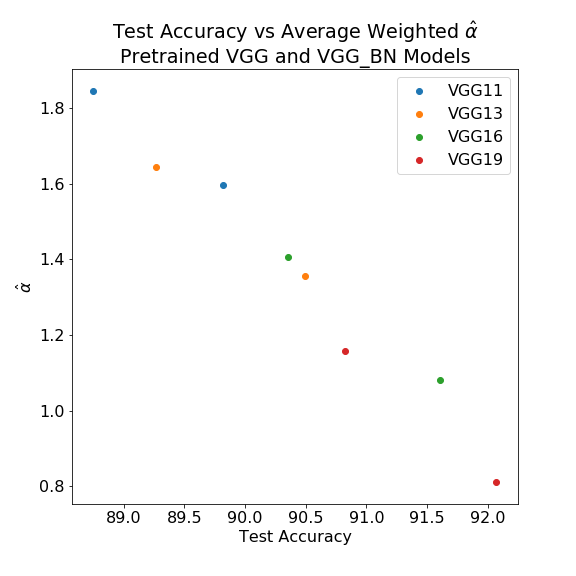
\includegraphics[scale=0.40]{img/vgg-w_alphas.png}
%% COMBINED WITH ABOVE %%    \caption{
%% COMBINED WITH ABOVE %% Pre-trained VGG and VGG BN Architectures and DNNs.  Test Accuracy and weighted average $\hat{\alpha}$ for
%% COMBINED WITH ABOVE %%  VGG11 vs VGG11\_BN ({\color{blue}{blue}}),
%% COMBINED WITH ABOVE %% VGG13 vs VGG13\_BN ({\color{orange}{orange}}),
%% COMBINED WITH ABOVE %% VGG16 vs VGG16\_BN ({\color{green}{green}}),  and
%% COMBINED WITH ABOVE %% VGG19 vs VGG19\_BN ({\color{red}{red}}). 
%% COMBINED WITH ABOVE %% }
%% COMBINED WITH ABOVE %%   \label{fig:vgg_alphahat}
%% COMBINED WITH ABOVE %% \end{figure}



\begin{table}[t]
\small
\begin{center}
\begin{tabular}{|p{1in}|c|c|c|c|c|c|c|}
\hline
Architecture 
 & Model &Top1 
 & Top5 & $L$ & $N_{\alpha}$ & $\hat{\alpha}$ \\
\hline
VGG11 & VGG11 & & & & & \\
  & VGG11 BN & & & & & \\
\hline
VGG13 & VGG13 & & & & & \\
  & VGG13 BN & & & & & \\
\hline
VGG16 & VGG16 & & & & & \\
  & VGG16 BN & & & & & \\
\hline
VGG19 & VGG19 & & & & & \\
  & VGG19 BN & & & & & \\
\hline
\end{tabular}
\end{center}
\caption{Results for VGG Series of Architectures and DNN Models.}
\label{table:models_VGG}
\end{table}



We start by looking at the VGG class of models, including VGG11, VGG13, VGG16, and VGG19, and their counterparts with Batch Normalization, VGG11\_BN, VGG13\_BN, VGG16\_BN and VGG19\_BN.  
See Figures~\ref{fig:vgg_lognorms} and~\ref{fig:vgg_alphahat} as well as Table~\ref{table:models_VGG} for details.
XXX.  SOME COMMENTS.

(((
As an example of our main results, consider Figure~\ref{fig:vgg}, which shows both the average log Frobenius norm 
($\langle\log\Vert\mathbf{W}\Vert_{F}\rangle$, defined in Eqn.~(\ref{eqn:av_log_norm}))
as well as the weighted average PL exponent ($\hat{\alpha}$, defined in Eqn.~(\ref{eqn:alpha_hat_specific}))
as a function of the reported (Top1) test accuracy for the series of pre-trained VGG models (available in the pyTorch package~\cite{pyTorch}).
(See Table~\ref{table:models_VGG} for additional details.)
Figure~\ref{fig:vgg_lognorms} shows the average log Frobenius norm results, which are quite good; and 
Figure \ref{fig:vgg_alphahat} shows the weighted average PL exponent results, which yield slight improvements due to the method we introduce.
Importantly, since we are using reported test accuracies (i.e., from the literature, and not due to the pecularities of our training), we did not need to retrain any models.
Equally importantly, we did not need to peek at the ImageNet test data to make this plot; and, in fact, we did not even need the ImageNet training data either.  
)))


\paragraph{ResNet Models.}

\begin{figure}[!htb]
   \centering
   \subfigure[log Frobenius norm $\langle\log\Vert\mathbf{W}\Vert_{F}\rangle$]{
      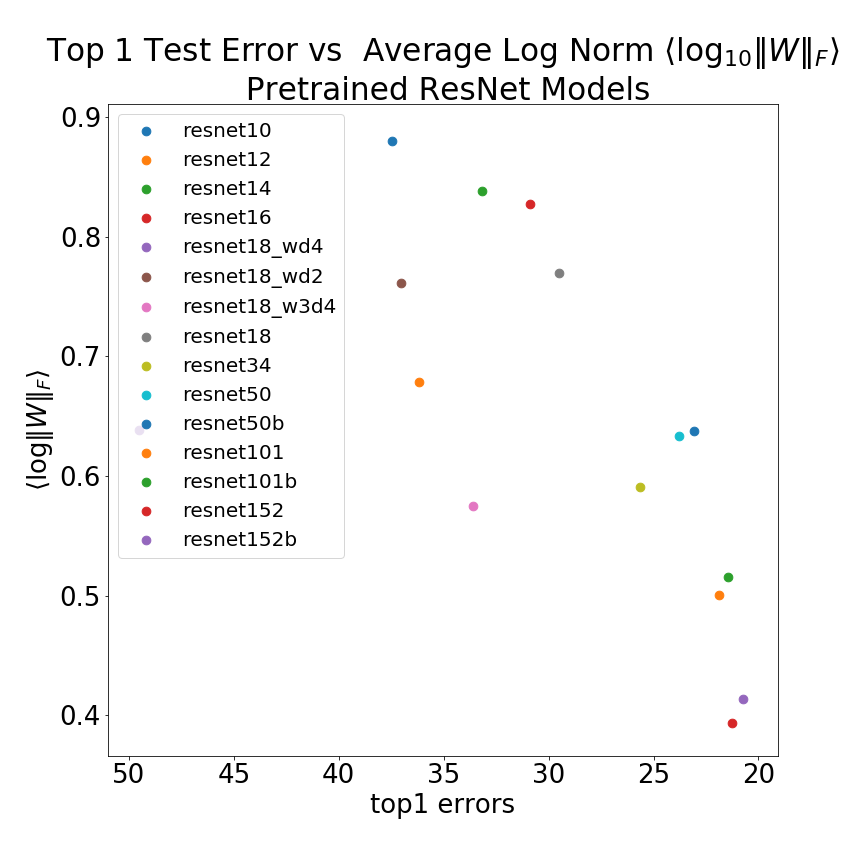
\includegraphics[scale=0.30]{img/ResNet_top1-lognorms.png}
      \label{fig:resnet_lognorms}
   }
   \subfigure[weighted average PL exponent $\hat{\alpha}$]{
      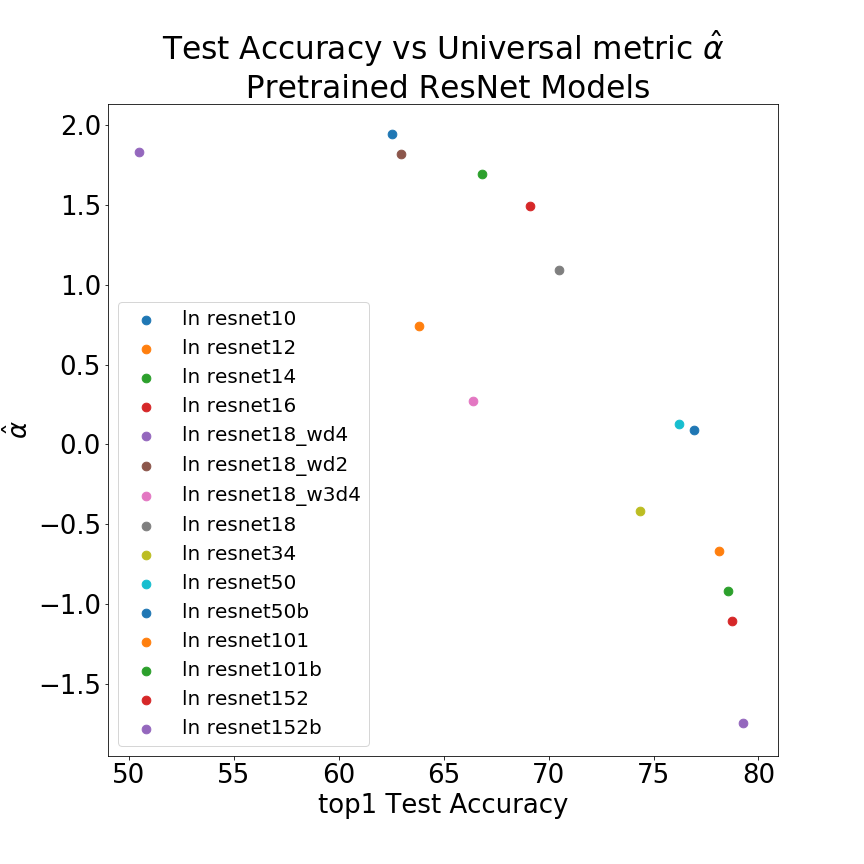
\includegraphics[scale=0.30]{img/ResNet-w_alphas.png}
      \label{fig:resnet_alphahat}
   }
   \caption{
      Pre-trained
      ResNet Series of Architectures and DNNs.  
      Top 1 Test error versus
      average log Frobenius norm $\langle\log\Vert\mathbf{W}\Vert_{F}\rangle$ (in (\ref{fig:resnet_lognorms}))
      or
      weighted average PL exponent $\hat{\alpha}$ (in (\ref{fig:resnet_alphahat})).
           }
   \label{fig:resnet}
\end{figure}

\begin{table}[!htb]
\small
\begin{center}
\begin{tabular}{|p{1in}|c|c|c|c|c|c|c|}
\hline
Architecture 
 & Model
 & Top 1 Error & $\hat{\alpha}$ \\
\hline
ResNet (small)  & resnet10 & 37.46 & \\
& resnet12 & 36.18 & \\
& resnet14 & 33.17 & \\
& resnet16 & 30.9 & \\
\hline
ResNet18 & resnet18\_wd4 & XX & \\
& resnet18\_wd2 & XX & \\
& resnet18 \_wd3d4& XX & \\
& resnet18 & XX & \\

\hline
ResNet34 & resnet34 & 25.66 & \\
\hline
ResNet50 & resnet50 & 23.79 & \\
& resnet50b &  & \\

\hline
ResNet101 & resnet101 & XX.XX & \\
& resnet101b & XX.XX & \\
\hline
ResNet152 & resnet152 & XX,XX & \\
& resnet152b & XX,XX & \\
\hline
\end{tabular}
\end{center}
\caption{Results for ResNet Series of Architectures and DNN Models.
         \michael{Are we going to have the same set of cols for ResNet at least that we had for VGG.}
        }
\label{table:models_resnet}
\end{table}

Next we look at the ResNet class of models. 
See
Figures~\ref{fig:resnet_lognorms}
and~\ref{fig:resnet_alphahat}
as well as
Table~\ref{table:models_resnet}
for details.
XXX.  SOME COMMENTS.


\paragraph{More Pre-trained Models.}

Here are results for more pre-trained models.
See
Table~\ref{table:models_more}
as well as 
Figure~\ref{fig:models_more} 
for details.
XXX.  SOME COMMENTS.

\begin{table}[!htb]
\small
\begin{center}
\begin{tabular}{|p{1in}|c|c|c|c|c|c|c|}
\hline
Architecture 
 & Model
 & Test Accuracy \\
\hline
GoogLeNet & & \\
\hline
ResNeXt & & \\
\hline
SqueezeNet & & \\
\hline
\end{tabular}
\end{center}
\caption{Results for more models.
         \michael{Why is this split off from the next table.}
        }
\label{table:models_more}
\end{table}

\begin{figure}[!htb]
   \centering
   \subfigure[DenseNet] {
       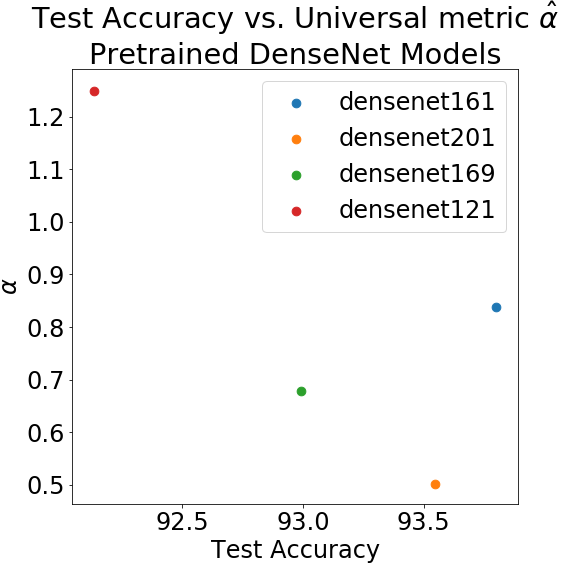
\includegraphics[scale=0.30]{img/densenet-pytorch-w_alphas.png} 
       \label{fig:densenet}
   }
   \subfigure[SqueezeNet]{
       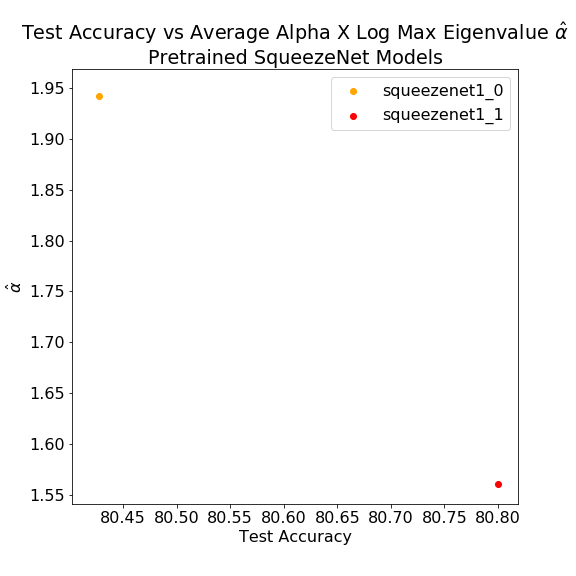
\includegraphics[scale=0.30]{img/squeezenet-pytorch-w_alphas.png} 
       \label{fig:squeezenet}
   }
   \caption{
      Pre-trained 
      Densenet and SqueezeNet PyTorch 
      Models.
      Test Accuracy versus
      $\hat{\alpha}$.
           }
   \label{fig:models_more}
\end{figure}


\paragraph{Still More Pre-trained Models.}

Here are results for still more pre-trained models.
See
Table~\ref{table:models_still_more}
as well as
Figures~\ref{fig:still_more_1} and \ref{fig:still_more_2}
for details.
XXX.  SOME COMMENTS.


\begin{table}[!htb]
\small
\begin{center}
\begin{tabular}{|p{1in}|c|c|c|c|c|c|c|}
\hline
Architecture 
 & Model
 & Top 1 Error \\
 \hline
 DenseNet & densenet121 & 25.57 & \\
& densenet161 & 22.86 & \\
& densenet169 & 24.4 & \\
& densenet201 & 23.1 & \\\hline
DPN & dpn68 & 24.17 & \\
& dpn98 & 20.81 & \\
& dpn131 & 20.54 & \\
\hline
MeNet & menet108\_8x1\_g3 & 43.92 & \\
& menet128\_8x1\_g4 & 43.95 & \\
& menet228\_12x1\_g3 & 33.57 & \\
& menet256\_12x1\_g4 & 33.41 & \\
& menet348\_12x1\_g3 & 30.1 & \\
& menet352\_12x1\_g8 & 33.31 & \\
& menet456\_24x1\_g3 & 28.4 & \\
\hline
MobileNet & mobilenet\_wd4 & 46.26 & \\
& mobilenet\_wd2 & 36.3 & \\
& mobilenet\_w3d4 & 33.54 & \\
& mobilenet\_w1 & 29.86 & \\
\hline
MobileNetV2 & mobilenetv2\_wd4 & 49.72 & \\
& mobilenetv2\_wd2 & 36.54 & \\
& mobilenetv2\_w3d4 & 31.89 & \\
& mobilenetv2\_w1 & 29.31 & \\
\hline
FDMobileNet & fdmobilenet\_wd4 & 55.77 & \\
& fdmobilenet\_wd2 & 43.85 & \\
& fdmobilenet\_w1 & 34.7 & \\
\hline
SE-ResNet & seresnet50 & 22.47 & \\
& seresnet101 & 21.88 & \\
& seresnet152 & 21.48 & \\
\hline
SE-ResNeXt & seresnext50\_32x4d & 21.0 & \\
& seresnext101\_32x4d & 19.96 & \\
\hline
ShuffleNet & shufflenetv2\_wd2 & 41.48 & \\
& shufflenetv2\_w1 & 34.39 & \\
\hline
\end{tabular}
\end{center}
\caption{Results for still more models.
         \michael{Why is this split off from previous table.}
         \michael{Why is CondenseNet missing.}
         \michael{Why Test Accuracy for others and Top 1 Error here.}
        }
\label{table:models_still_more}
\end{table}


\begin{figure}[!htb]
   \centering
   \subfigure[CondenseNet]{
       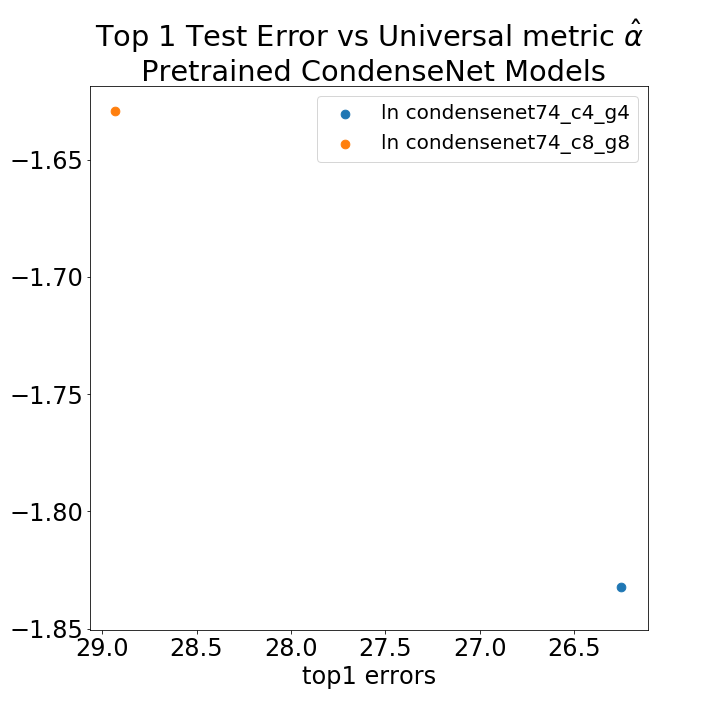
\includegraphics[scale=0.19]{img/CondenseNet-w_alphas.png} 
       \label{fig:densenet-small}
   }
   \subfigure[DPN]{
       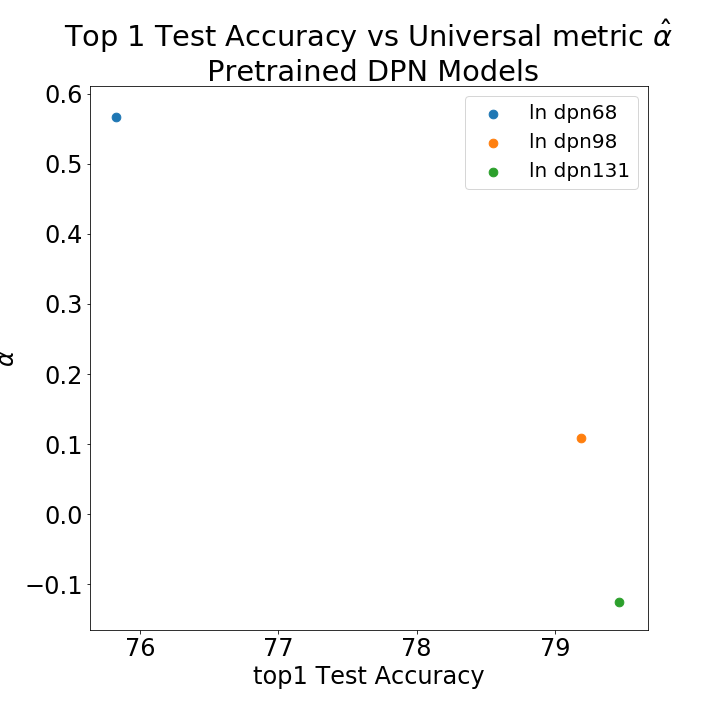
\includegraphics[scale=0.19]{img/DPN-w_alphas.png} 
       \label{fig:dpn-net}
   }
   \subfigure[ShuffleNet]{
      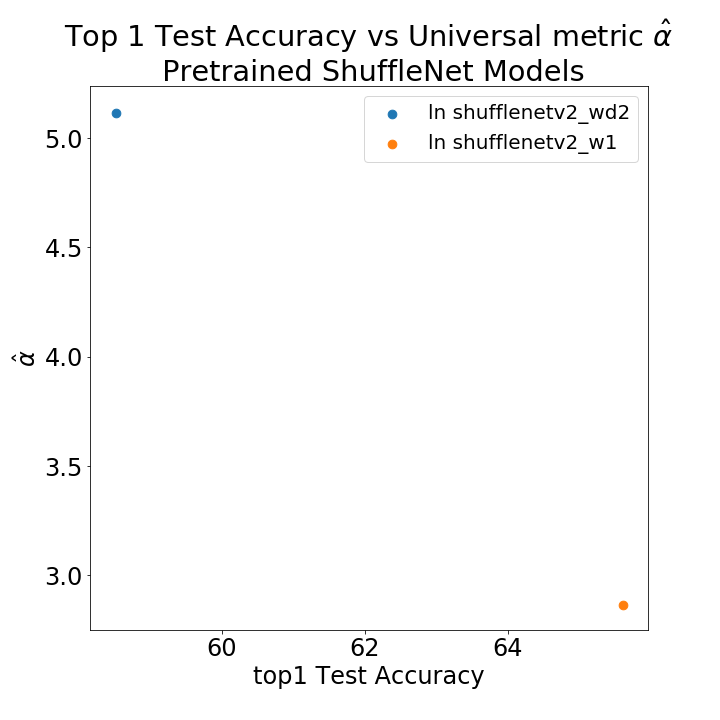
\includegraphics[scale=0.19]{img/ShuffleNet-w_alphas.png}
      \label{fig:shufflenet-small}
   }
   \caption{
      Pre-trained 
      CondenseNet, DPN, and ShuffleNet
      Models.
      Top 1 Test error versus
      $\hat{\alpha}$.
           }
   \label{fig:still_more_1}
\end{figure}


\begin{figure}[!htb]
   \centering
   \subfigure[MobileNet]{
      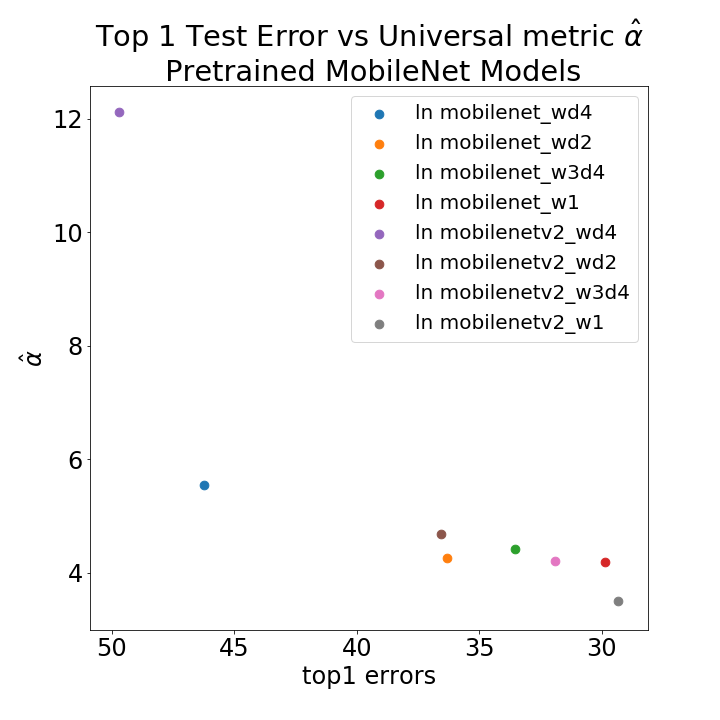
\includegraphics[scale=0.19]{img/MobileNet-w_alphas.png} 
      \label{fig:resnet-small}
   }
   \subfigure[SeResNet]{
      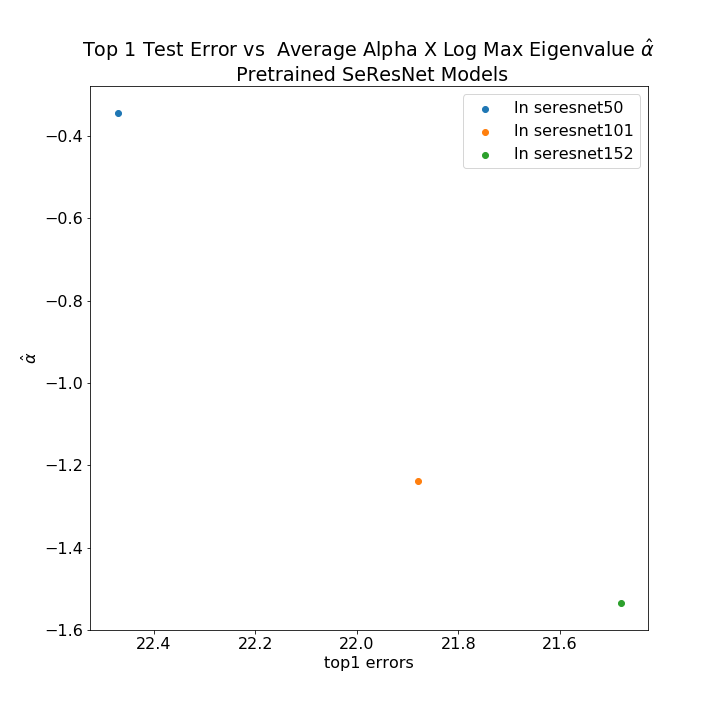
\includegraphics[scale=0.19]{img/SeResNet-w_alphas.png}
      \label{fig:shufflenet-small}
   }
   \subfigure[SeResNeXt]{
      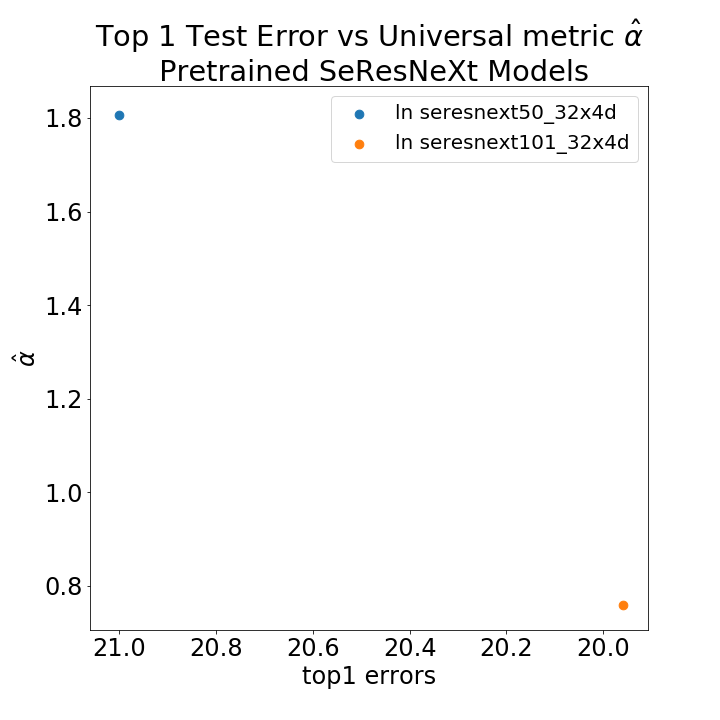
\includegraphics[scale=0.19]{img/SeResNeXt-w_alphas.png}
      \label{fig:shufflenet-small}
   }
   \caption{
      Pre-trained 
      MeNet, SeResNet, and SeResNeXt
      Models.
      Top 1 Test error versus
      $\hat{\alpha}$.
           }
   \label{fig:still_more_2}
\end{figure}


\paragraph{Counterexamples.}
There are of course exceptions here and there.
See
Figure~\ref{fig:counter-examples}
as well as 
Table~\ref{table:models_still_more}
for details on the counterexamples.
XXX.  COMMENTS.

\begin{figure}[!htb]
   \centering
   \subfigure[ResNeXt]{
      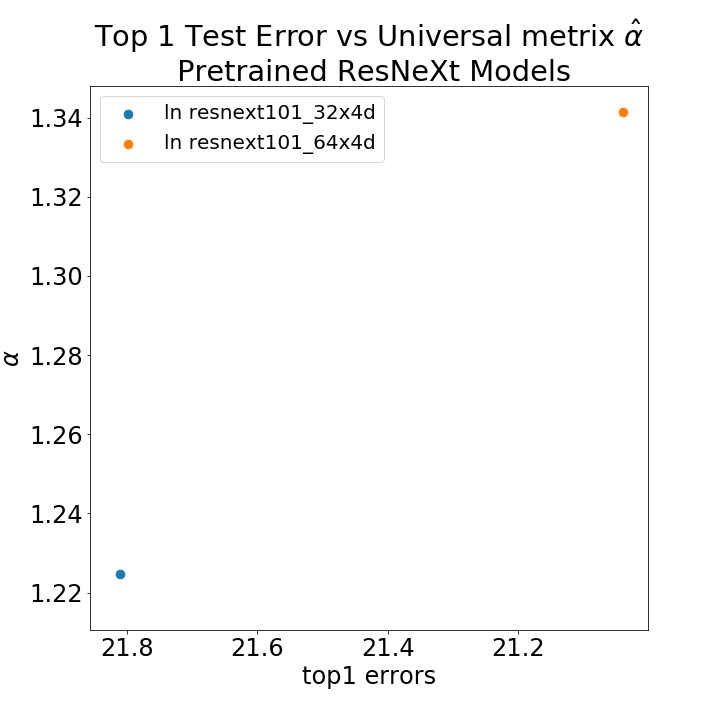
\includegraphics[scale=0.19]{img/ResNeXt-w_alphas.png} 
      \label{fig:resnet-small}
   }
   \subfigure[MeNet]{
      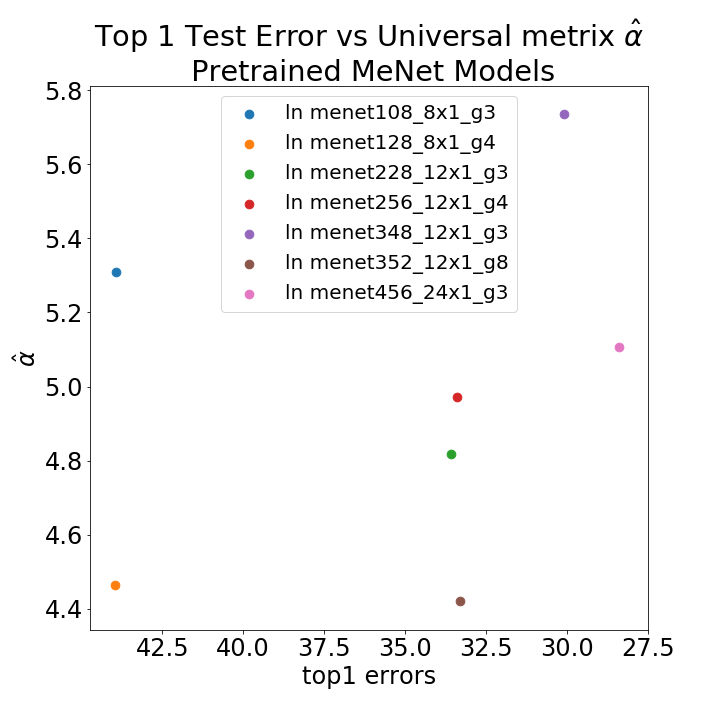
\includegraphics[scale=0.19]{img/MeNet-w_alphas.png} 
      \label{fig:menet-net}
   }
   \subfigure[FDMobileNet]{
      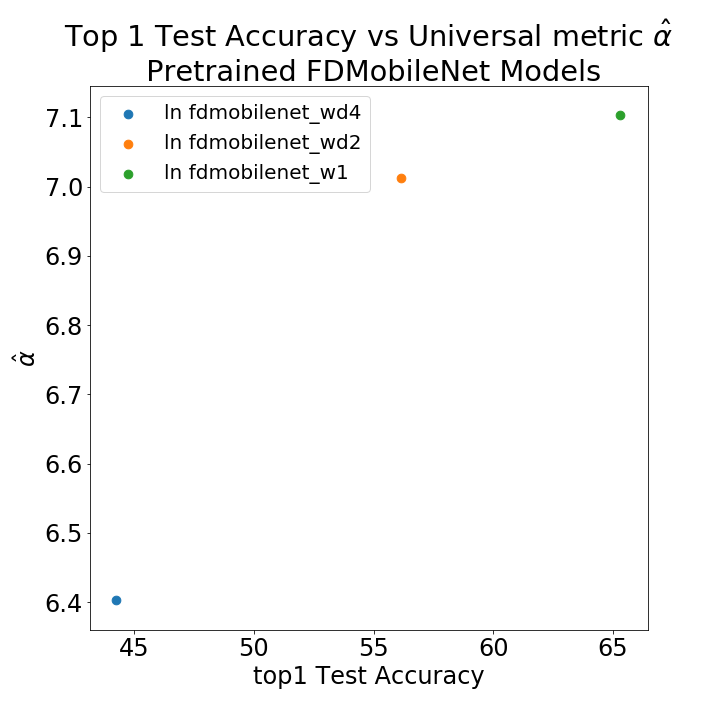
\includegraphics[scale=0.19]{img/FDMobileNet-w_alphas.png} 
      \label{fig:resnet-small}
   }
   \caption{
      Pre-trained 
      ResNeXt, MeNet, and FDMobileNet
      Models 
      that provide counterexamples to our main trends.
      Top 1 Test error versus
      $\hat{\alpha}$.
           }
   \label{fig:counter-examples}
\end{figure}


